
\begin{frame}{Why can topic modeling do for grants?}
  \begin{itemize}
    \item Discover research areas without supervision
    \item Discover research domains at various resolutions
    \item Map trends over time
  \end{itemize}
\end{frame}

\begin{frame}{Research Areas}
  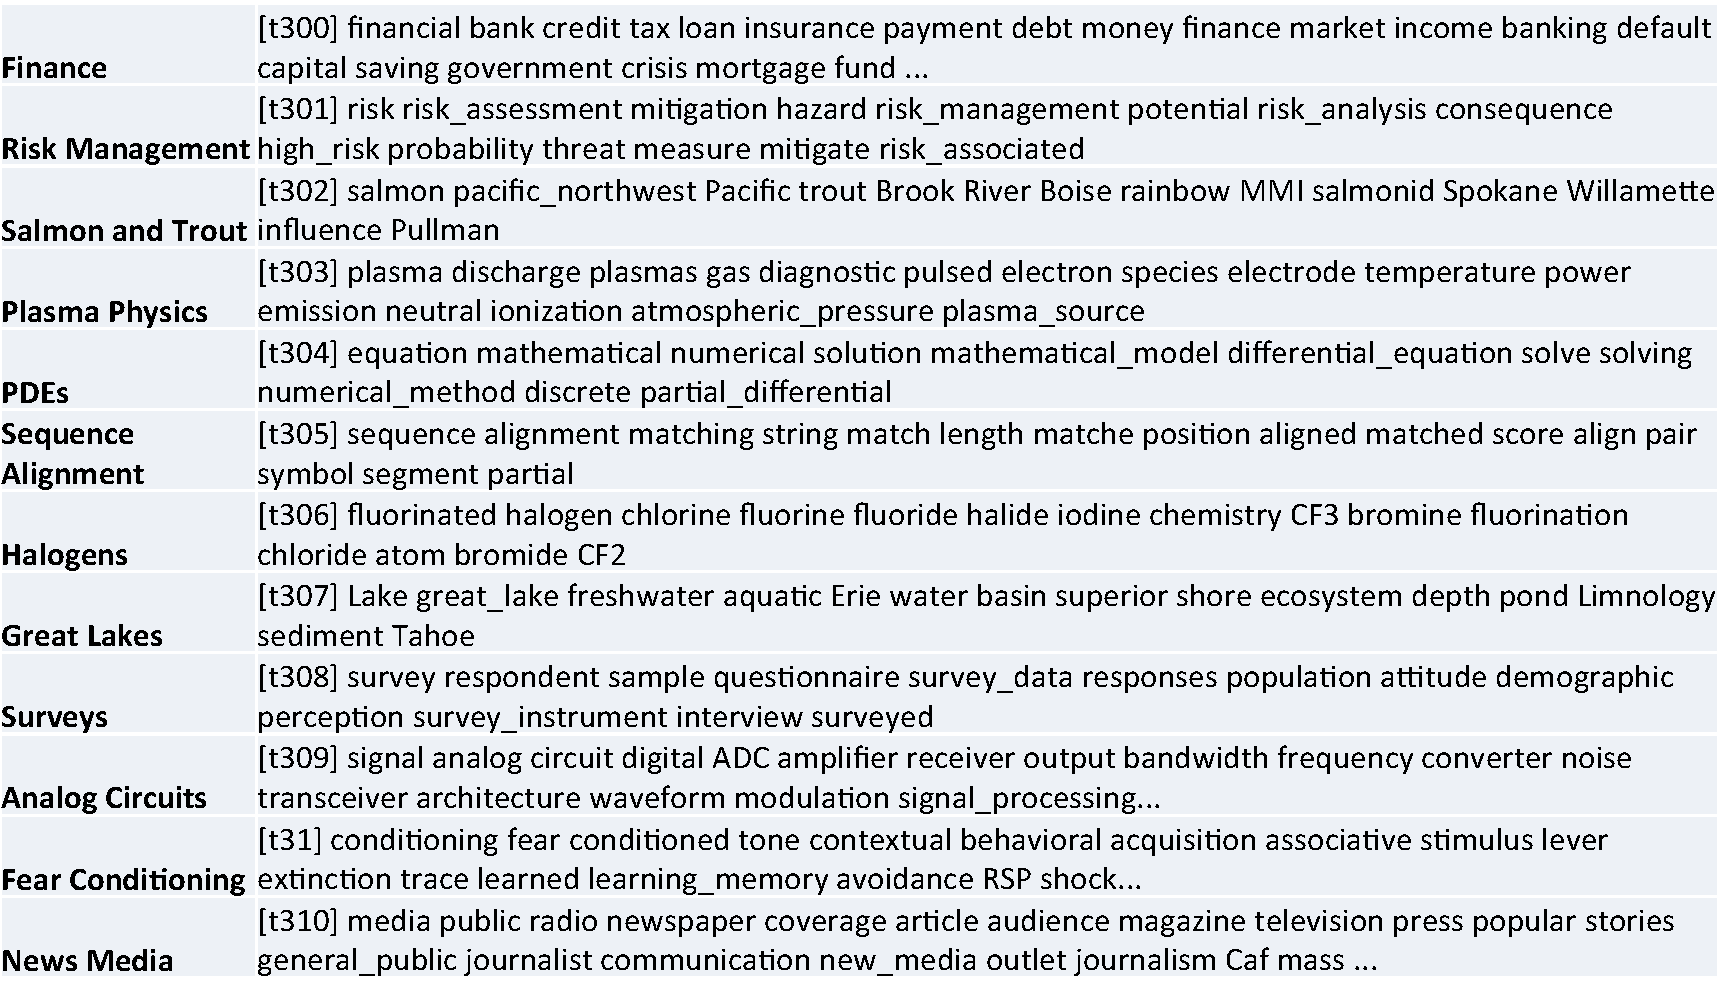
\includegraphics[width=1.0\linewidth]{topic_models/nsf_topics} \\
  \pause
  \centering
  Names added as \emph{post hoc} analysis
\end{frame}

\begin{frame}{Research Areas}
  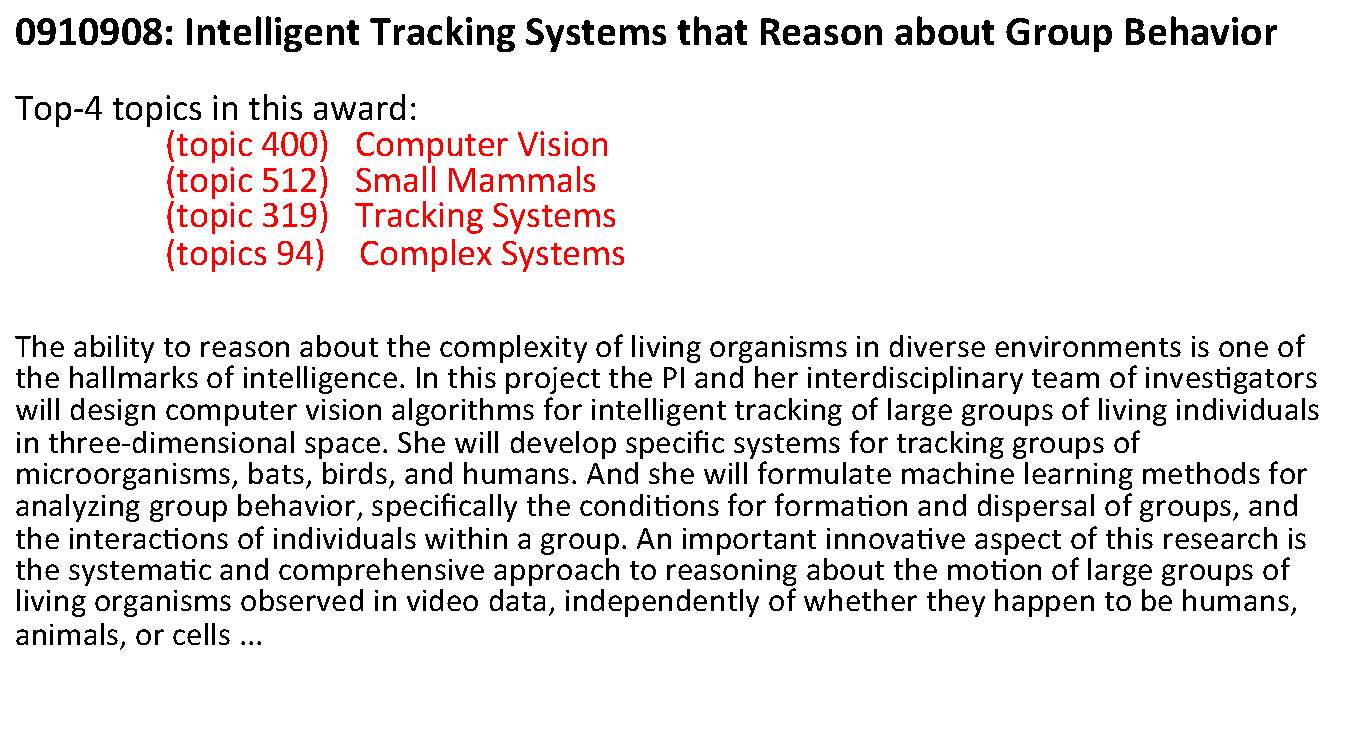
\includegraphics[width=1.0\linewidth]{topic_models/nsf_topic_ex}
\end{frame}

\begin{frame}{Resolutions}
  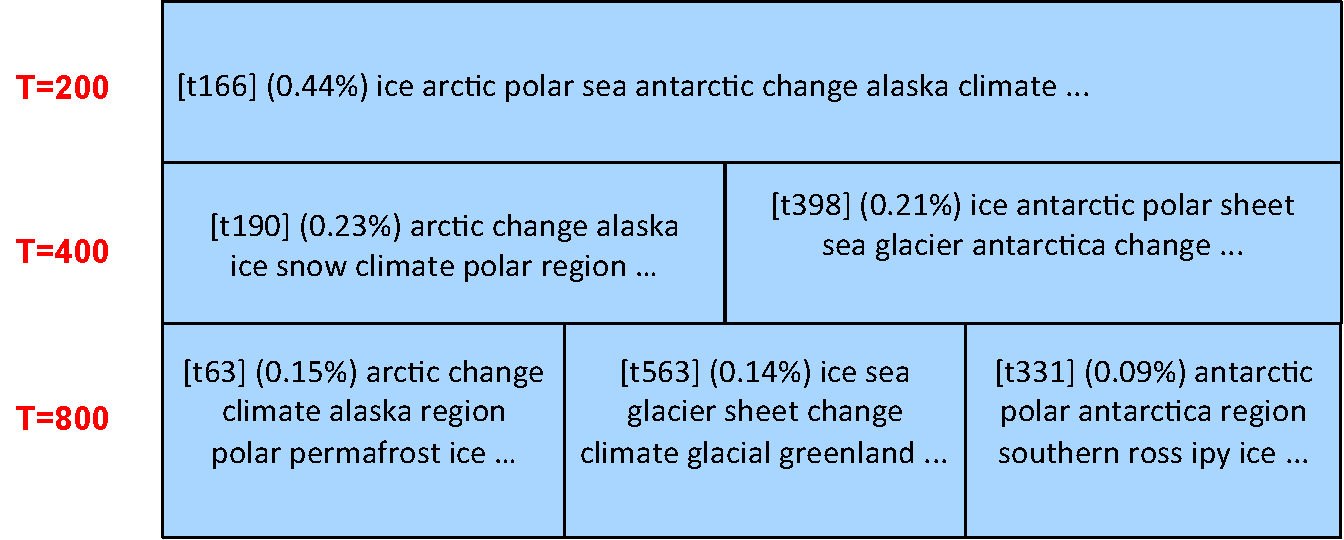
\includegraphics[width=1.0\linewidth]{topic_models/nsf_resolution}
\end{frame}

\begin{frame}{Trends over Time}
  \begin{columns}
    \column{.5\linewidth}
      \begin{block}{Angiogensis Topic}
        Technique for creating new blood vessels.
      \end{block}
      Publications lag behind funding.
  \centering
    \column{.5\linewidth}  
  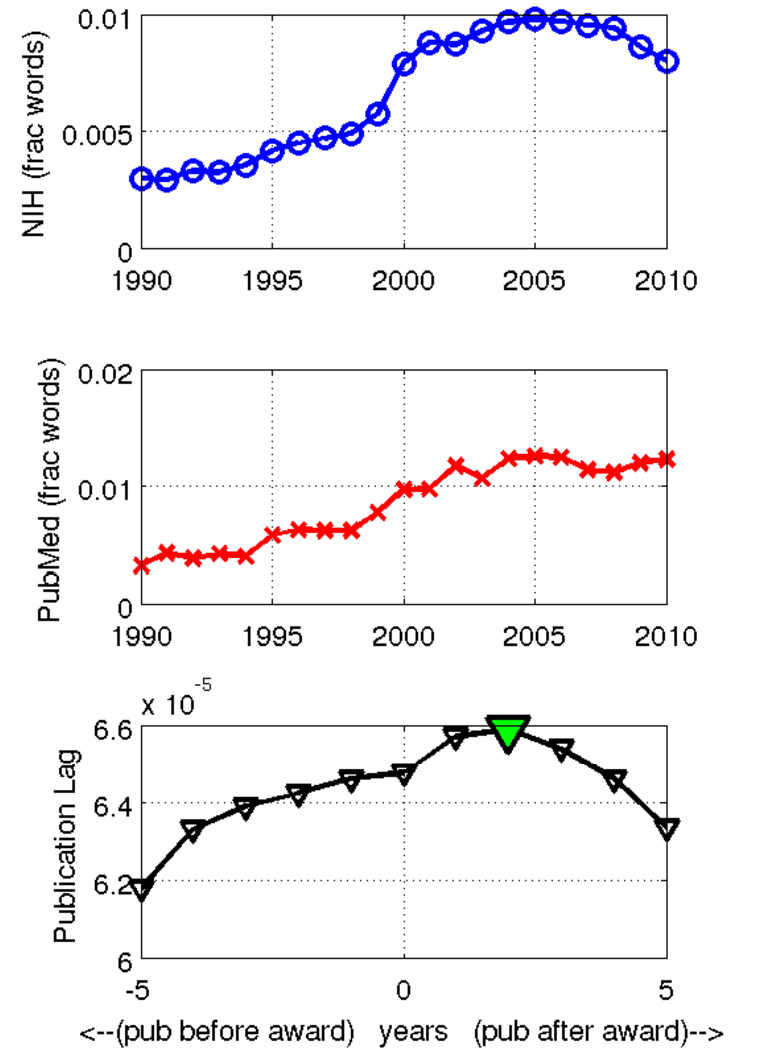
\includegraphics[width=1.0\linewidth]{topic_models/publication_lag}
  \end{columns}
\end{frame}

\begin{frame}{Trends over Time}
  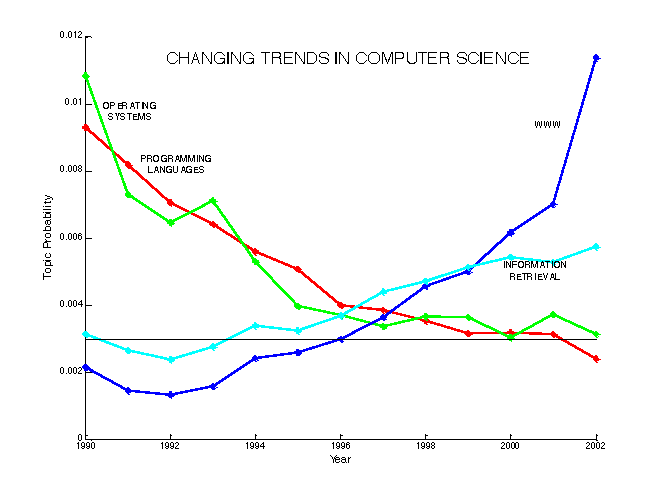
\includegraphics[width=1.0\linewidth]{topic_models/cs_trends}
\end{frame}

\begin{frame}{Comparing Portfolios}
  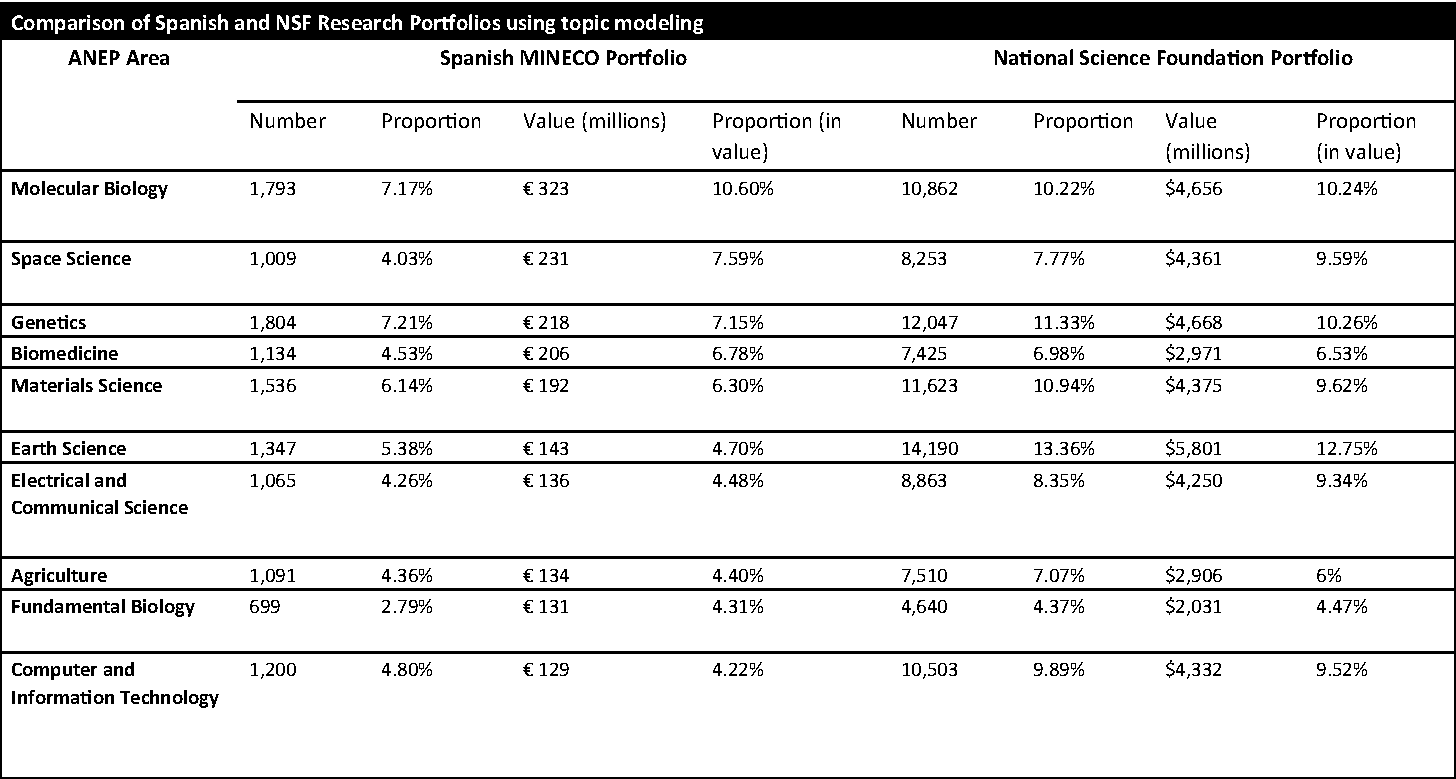
\includegraphics[width=1.0\linewidth]{topic_models/spain_comparison}
\end{frame}

\begin{frame}{What can't topic modeling do for grants?}
  \begin{itemize}
    \item Map research into pre-defined taxonomies 
      \begin{itemize}
        \item Supervised methods: \textsc{svm}, decision trees, information retrieval
      \end{itemize}
    \item Summarize research beyond a ``bag of words''
      \begin{itemize}
        \item Extractive summarization
      \end{itemize}      
    \item Use metadata to {\bf discover} topics 
      \begin{itemize}
        \item Network models
      \end{itemize}
  \end{itemize}
\end{frame}
